% ---------------------------------------------------------------------------
% VCBM 2026 poster abstract (dynamic functional connectivity in ABIDE)
% Authored from the EG/VCBM 2026 template (EGauthorGuidelines-vcbm2026-conference.tex).
% Do not edit the class/style/bst files; this file is the manuscript.
% ---------------------------------------------------------------------------

\documentclass{egpubl-eurovis-short}
\usepackage{vcbm2026-conference}

% --- for VCBM 2026
\WsSubmission    % submission to VCBM (poster track)
%\WsPaper        % uncomment for the final (camera-ready) version

\electronicVersion

% !! *please* don't change anything above unless you REALLY know what you are doing
% ------------------------------------------------------------------------

\ifpdf \usepackage[pdftex]{graphicx} \pdfcompresslevel=9
\else \usepackage[dvips]{graphicx} \fi

\graphicspath{ {./figures/} }

\PrintedOrElectronic

\usepackage{t1enc,dfadobe}
\usepackage{egweblnk}
\usepackage{cite}

\usepackage{tikz}
\usetikzlibrary{arrows.meta,positioning}
\usepackage{orcidlink}

% Render the classification block in the modern "CCS Concepts" style used by
% recent VCBM posters, instead of the legacy "Categories and Subject
% Descriptors (ACM CCS)" label provided by the class.
\makeatletter
\def\classification{\vskip 5.5pt\par\reset@font\rmfamily\textbf{CCS Concepts}\\}
\def\endclassification{\relax}
\makeatother

% ------------------------------------------------------------------------

\title[Dynamic Functional Connectivity visualization of ABIDE]%
      {Interactive Visualization of Dynamic Functional Connectivity\\
       in the ABIDE Autism Dataset}

% Placeholder author block -- replace with final authors/affiliations.
\author[D. Eliad et al.]
       {D. Eliad$^{1}$
        and S. Schielen\,\orcidlink{0009-0005-1223-0449}$^{1}$
        and A. Aldenkamp\,$^{1}$
        and D. Ruijters\,\orcidlink{0000-0002-9931-4047}$^{1\,2}$
        and S. Zinger\,\orcidlink{0000-0001-9357-3067}$^{1}$
        \\
        $^1$Department of Electrical Engineering, Eindhoven University of Technology, Eindhoven, The Netherlands\\
$^2$Department of Neurology, Maastricht
University Medical Center, Maastricht, The
Netherlands}


% ------------------------------------------------------------------------
\begin{document}

\teaser{
  \centering
  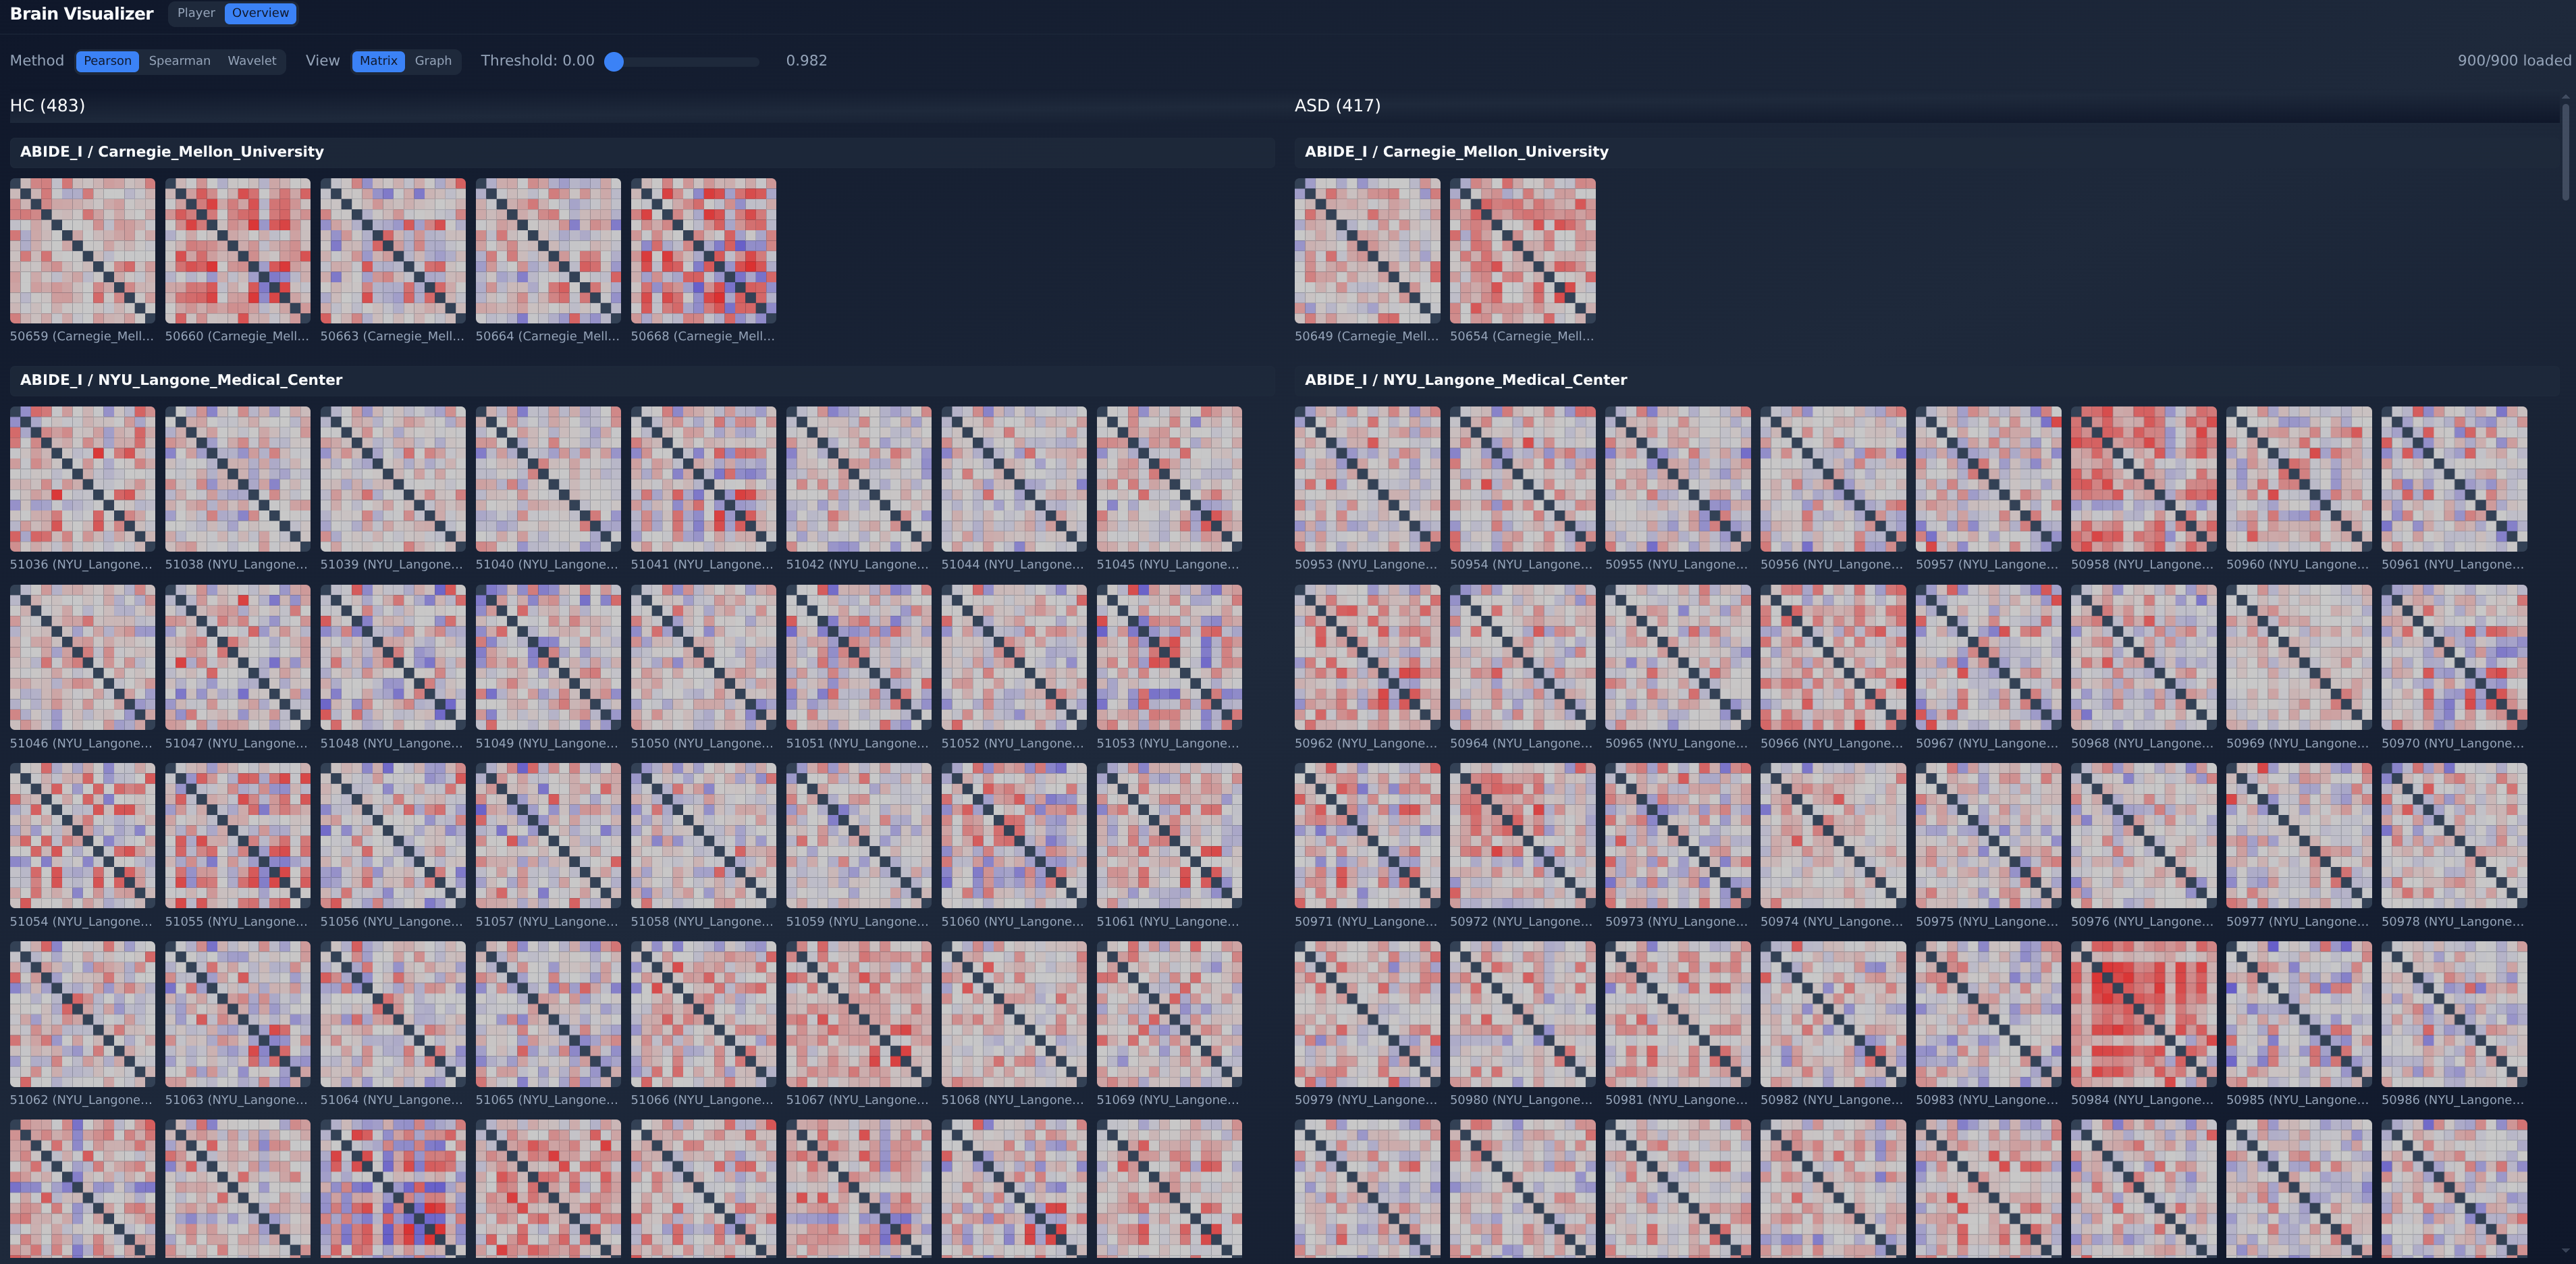
\includegraphics[width=0.8\linewidth]{overview.png}
  \caption{\label{fig:overview}
    Overview tab: per subject connectivity matrix split into control ($N=483$) and ASD ($N=417$) classes grouped by acquisition site.}
}

\maketitle

\begin{abstract}
Autism spectrum disorder (ASD) is currently diagnosed using observation-based criteria, while an objective test is desired~\cite{schielen-2024}. Resting state functional connectivity between brain regions is increasingly understood to be a dynamic process, varying in time~\cite{hutchison-2013,preti-2016}. However, the tools currently available collapse a recording into a single correlation matrix and discard the time variations. We present an interactive web application for exploring the time varying functional connectivity between brain regions in the large ABIDE I+II autism fMRI dataset. Each recording is decomposed into resting state networks whose dynamic connectivity is measured over a sliding window using several methods, including wavelet lead coherence, a directional measure of which network leads which. These connections are visualized as a video of a graph with weighted edges, alongside a complementary overview pane to compare individual scans, or one diagnostic class against the other. This system turns a large, otherwise opaque dataset into a visual format for discovering time varying functional connectivity patterns. It is a step toward an interpretable neuroimaging tool that may aid diagnosis.

   \begin{classification}
    $\bullet$ \emph{Information systems} $\rightarrow$ 
Information systems applications $\rightarrow$ Decision support systems $\rightarrow$ Data analytics
   \end{classification}
\end{abstract}

%-------------------------------------------------------------------------
\section{Introduction}

Resting state fMRI (rs-fMRI) is the most studied imaging method in autism spectrum disorder (ASD) research~\cite{schielen-2024}, and the functional connectivity it reveals is central to studying the condition. This connectivity is conventionally computed over an entire recording, resulting in a single static connectivity matrix. However, dynamic functional connectivity captures information that static correlations discard~\cite{chang-2009}, and has shown promise as a biomarker for the diagnosis of autism~\cite{bernas-2017}, depression~\cite{cirstian-2023,pilmeyer-2024}, and cognitive aging~\cite{bernas-2021}. 

The Autism Brain Imaging Data Exchange (ABIDE) is a large, multisite rs-fMRI dataset. Recent work preprocessed ABIDE~I+II using independent component analysis (ICA) into resting state networks (RSNs) for 900 subjects (417~ASD, 483~controls)~\cite{schielen-2025}. ABIDE is the most comprehensive fMRI ASD dataset~\cite{schielen-2024} and is an ideal dataset for this dynamic functional connectivity visualization. However, common connectivity visualizers are static and lack the interactive, time varying exploration needed to understand dynamic patterns. We present a novel web application that fills this gap with an animated graph view of windowed connectivity between 14 RSNs, computed per subject from configurable parameters using symmetric correlations and a directional wavelet lead coherence measure, alongside a comparative overview across diagnostic classes and specific sites.


%-------------------------------------------------------------------------
\section{Neuroimaging and Brain Connectivity}
From group independent component analysis (ICA), 14 resting-state networks were identified~\cite{schielen-2025}. Functional connectivity between two networks is quantified by correlating their time series. Correlating the time series using a fixed length sliding window produces a series of matrices that describe the dynamic functional connectivity~\cite{hutchison-2013,preti-2016}.

The system offers three correlation measures. Pearson and Spearman correlation produce symmetric
matrices in the range $[-1,1]$. The third is a directional (asymmetric) measure, called wavelet lead coherence. The wavelet transform decomposes each signal into time and frequency, capturing how its frequency content varies over time rather than averaging over the whole scan. Wavelet coherence then acts as a localized correlation coefficient between two signals, and its cross-wavelet phase angle gives their lead or lag at each point in time and frequency~\cite{grinsted-2004,torrence-1998,chang-2009}, classifying each network pair as in-phase, anti-phase, leading, or lagging~\cite{bernas-2017,cirstian-2023}. The wavelet lead coherence measure reports values in the range $[0,1]$, the fraction of time and frequency points at which one network leads the other, computed in both directions, so the resulting matrix is asymmetric. This directional measure of correlation highlights lead and lag patterns that are consistent with causal influence and may motivate further research into causal relationships between networks~\cite{cirstian-2023}.

%-------------------------------------------------------------------------
\section{Visualizations of Dynamic Brain Activity}

\begin{figure}[tb]
  \centering
  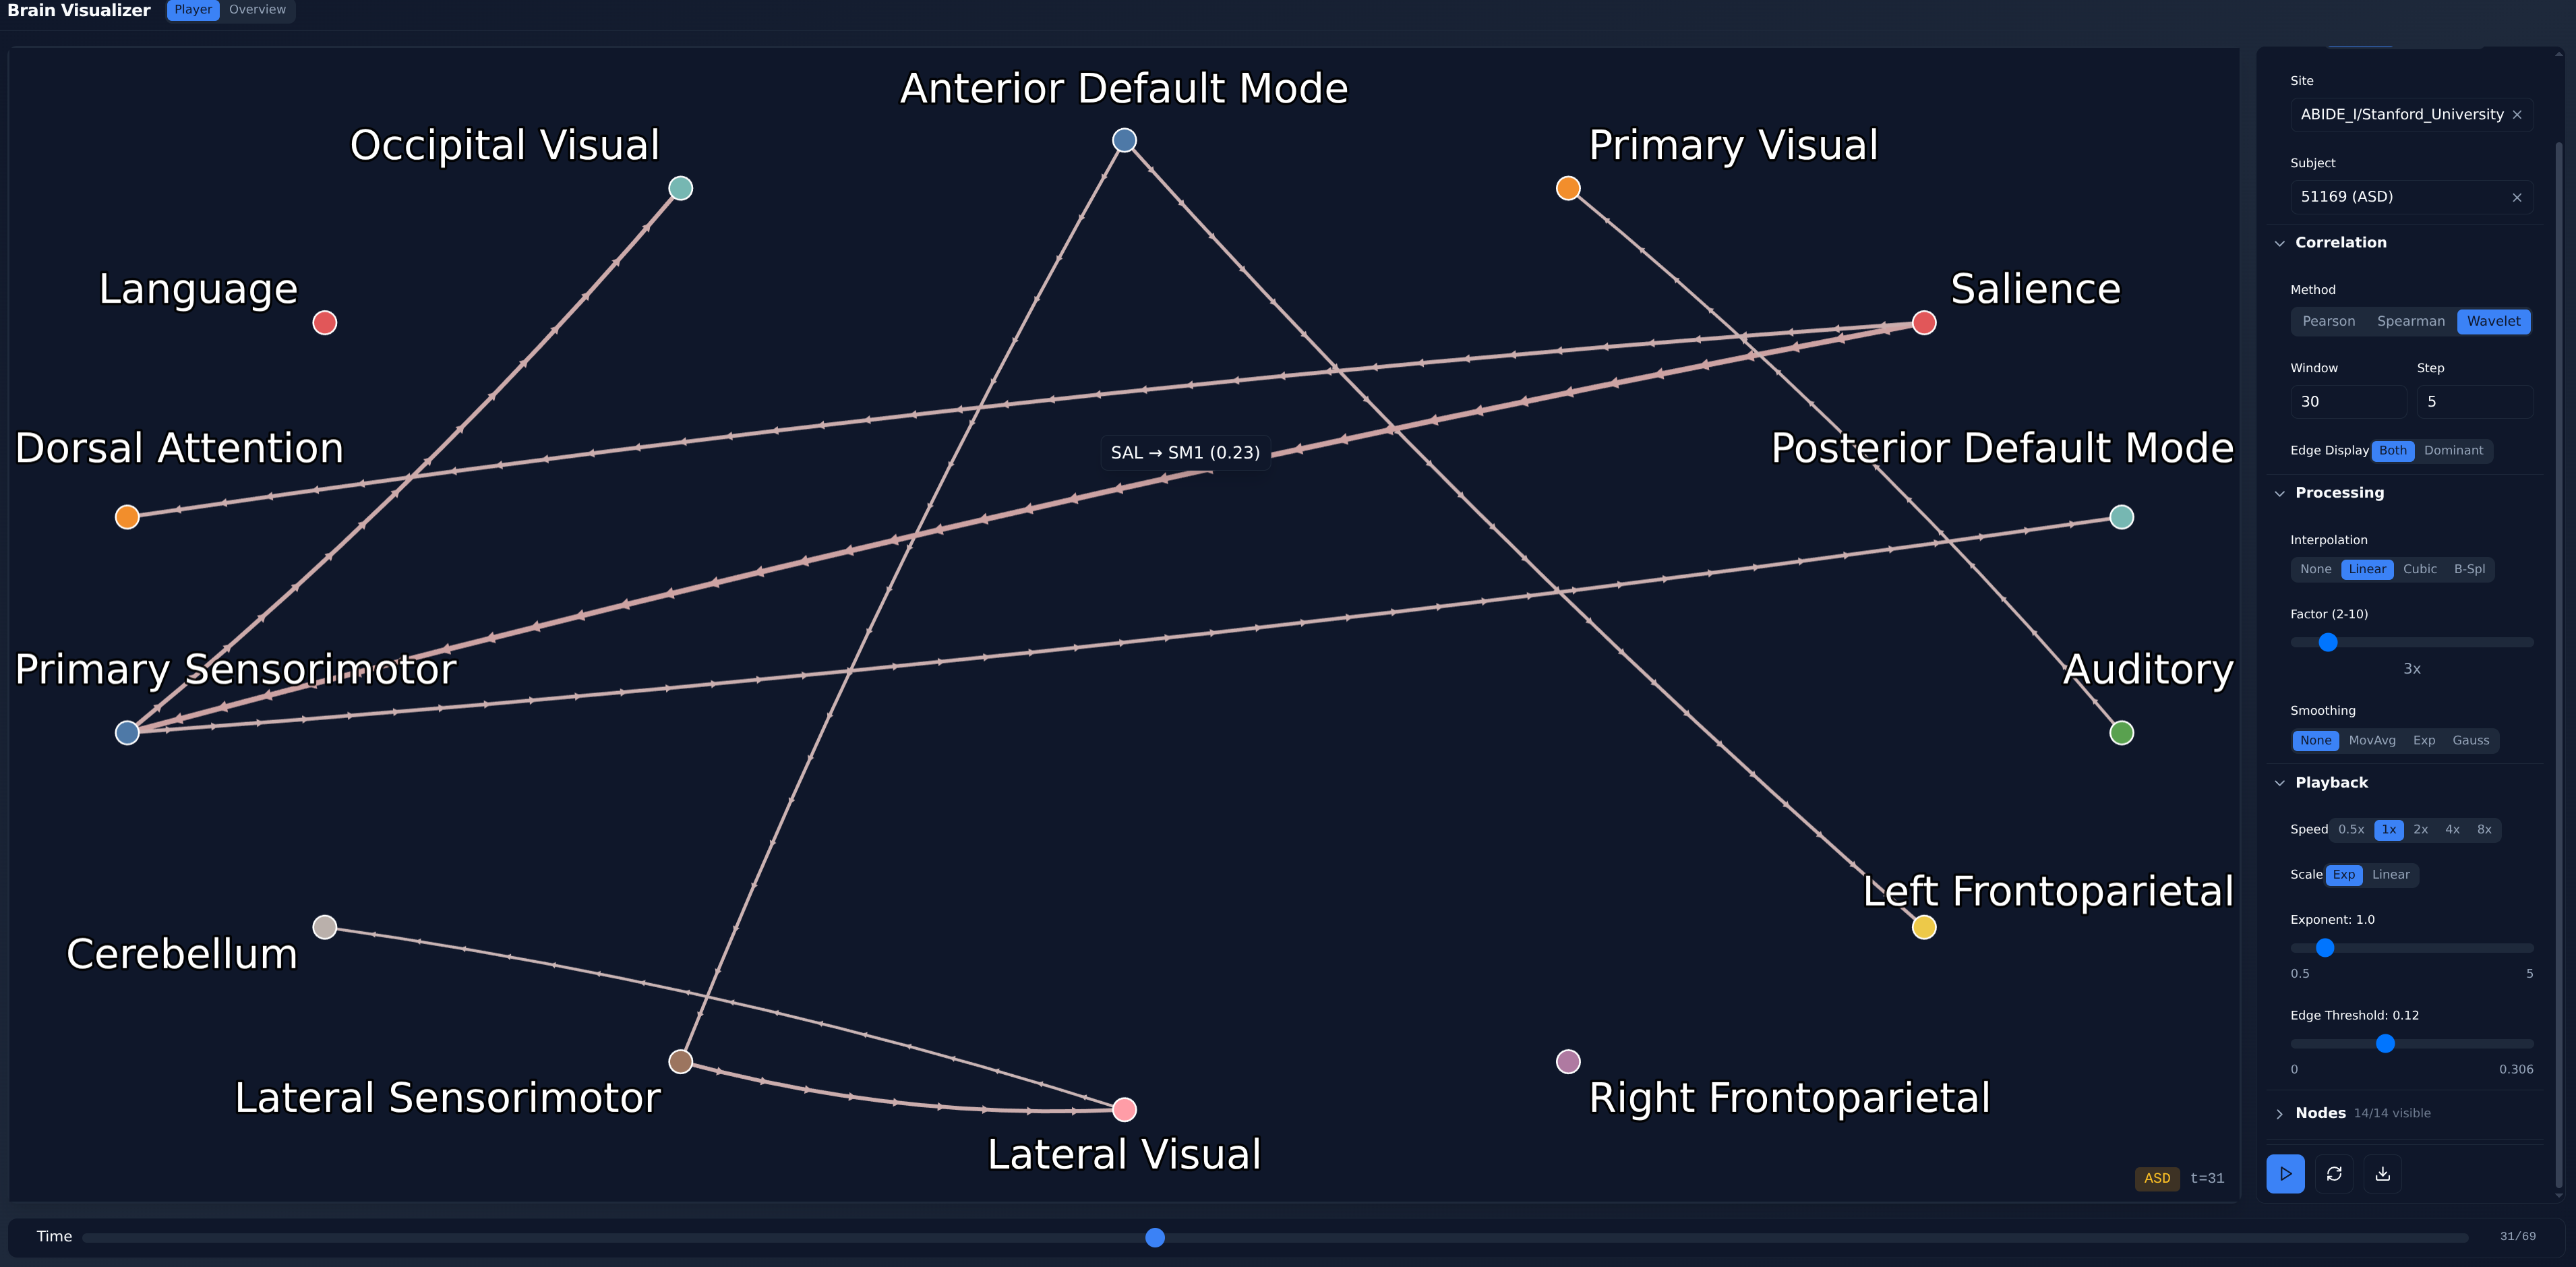
\includegraphics[width=\linewidth]{graph-view.png}
  \caption{\label{fig:graph}
    Graph view: 14 resting state networks on a ring with the current window's connectivity
    drawn as edges, where color encodes each correlation value and thickness encodes its magnitude.}
\end{figure}

The graph view places the resting state networks on a ring and draws the current frame's
connectivity matrix as edges (Figure~\ref{fig:graph}). The color of an edge encodes the correlation value
on a blue to red scale and thickness encodes its absolute magnitude. A configurable threshold
is used to hide weak edges and denoise the visualization. For wavelet lead coherence, the edges carry arrows showing the directionality of the correlation. The frames are animated over time, showing how the graph changes. Hovering over a network node isolates its edges, and hovering over an edge shows the two networks it connects and their connectivity correlation value. This view can also play aggregate sequences, the mean or median over all ASD or all control subjects, so an individual's dynamics can be compared against the mean or median of either class.

A complementary overview (Figure~\ref{fig:overview}) reduces each subject to a single correlation matrix over the entire recording, shown as a heatmap or a miniature graph, separated into healthy control and ASD columns and grouped by acquisition site. Read against the class mean and median, the overview enables fast scanning for individual outliers, group contrasts, and site variation. Identifying site variation and measurement error induced outliers is especially important, as it is a known confound in multisite rs-fMRI~\cite{schielen-2024}.

%-------------------------------------------------------------------------
\section{Conclusions}

Exploring dynamic functional connectivity of RSNs is a promising method for discovering explainable diagnostic features for the objective diagnosis of conditions such as ASD, but the dynamic patterns are difficult to observe with the static visualization tools currently available. Our contribution is a novel visualization tool for observing dynamic functional connectivity patterns between RSNs, publicly available at \URL{https://brainviz.ideabattery.org/}. Our system visualizes the large autism fMRI dataset ABIDE~I+II, enabling interactive exploration of each subject's RSN connectivity over time. This is a step toward translating high-dimensional fMRI features into interpretable information that can aid clinicians and produce explainable features for training machine learning models. Planned work adds a quantitative comparison of ASD against control subjects, turning exploratory observations into testable group differences and diagnostic features.

%-------------------------------------------------------------------------
\bibliographystyle{eg-alpha-doi}
\bibliography{brainviz}

\end{document}
